% Chapter 1

\chapter{Introducción general} % Main chapter title

\label{Chapter1} % For referencing the chapter elsewhere, use \ref{Chapter1} 
\label{IntroGeneral}

%----------------------------------------------------------------------------------------

% Define some commands to keep the formatting separated from the content 
\newcommand{\keyword}[1]{\textbf{#1}}
\newcommand{\tabhead}[1]{\textbf{#1}}
\newcommand{\code}[1]{\texttt{#1}}
\newcommand{\file}[1]{\texttt{\bfseries#1}}
\newcommand{\option}[1]{\texttt{\itshape#1}}
\newcommand{\grados}{$^{\circ}$}

%----------------------------------------------------------------------------------------

%\section{Introducción}

%----------------------------------------------------------------------------------------
\section{Introducción}

\subsection{La Internet de las Cosas y las formaciones ferroviarias}


La Internet de las Cosas (\textit{IoT}, por sus siglas en inglés) es una tecnología que se ha convertido en una tendencia en la actualidad. Este concepto se estableció en el mercado en la década de 1990, aunque su verdadero auge comenzó en los últimos años gracias a la aparición de dispositivos interconectados y al aumento en el uso de internet. La IoT se enfoca en la interconexión de objetos cotidianos con la red, lo que permite recopilar datos en tiempo real, optimizar procesos y tomar decisiones basadas en la información recolectada. Algunos beneficios que la IoT ofrece son una mayor eficiencia, una reducción de costos, un mejor monitoreo y control, y una mejor calidad de vida para las personas.

En el sector ferroviario, la IoT ha demostrado ser una tecnología clave para mejorar la eficiencia y la seguridad de las formaciones ferroviarias. Las formaciones ferroviarias pueden ser equipadas con sensores y dispositivos interconectados que permiten recopilar información sobre la ubicación, velocidad, consumo de energía, estado mecánico y otros aspectos importantes. Esta información se puede enviar en tiempo real a la red, lo que permite una mejor gestión del tráfico ferroviario y una toma de decisiones más rápida y eficaz. Además, la IoT también puede ayudar a prevenir accidentes ferroviarios al detectar problemas mecánicos antes de que se conviertan en un riesgo para la seguridad.


\vspace{1cm}

\begin{figure}[htpb]
	\centering
	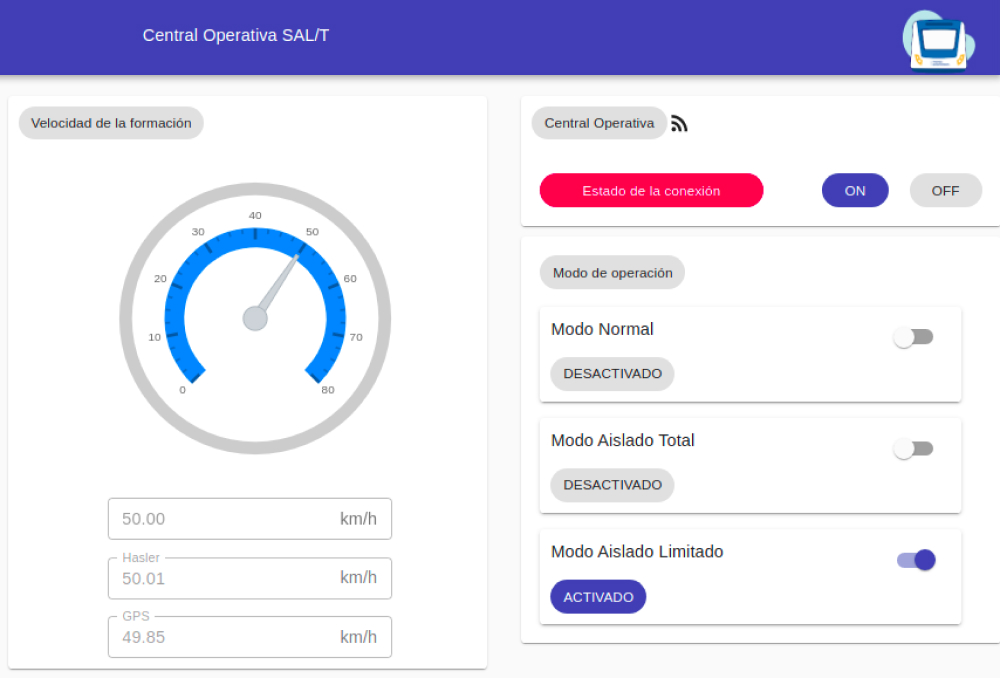
\includegraphics[width=.75\textwidth]{./Figures/dashboard.jpeg}
	\caption{Panel de control de la Central Operativa SAL/T para la visualización de datos en tiempo real.}
	\label{fig:dashboard}
\end{figure}


\subsection{Motivación}

El sistema ferroviario de la República Argentina cuenta con una gran cantidad de formaciones ferroviarias en las que se encuentran diferentes sistemas de seguridad a bordo. Estos equipos se encargan de supervisar el correcto funcionamiento de los subsistemas críticos. Ante una falla en uno de los subsistemas, una formación ferroviaria se detiene inmediatamente por la activación automática de las señales de corte de tracción (\textit{CT}) y frenado de emergencia (\textit{FE}). En esta situación, el conductor debe llevar la formación a un lugar seguro para que los pasajeros puedan descender y, posteriormente, trasladarla a un taller para que pueda ser reparada.

El \textit{SAL/T}, según sus siglas, Sistema de Aislamiento Limitado y Total [1], es un dispositivo del cual se cuenta con una primera versión prototipada; que se presenta como solución a las contingencias descritas anteriormente. De esta manera, el maquinista de una formación ferroviaria cunta con la posibilidad de activar y desactivar el \textit{modo aislado limitado}. En este modo, el equipo permite la circulación de la formación al desactivar las señales de corte de tracción y freno de emergencia generadas por los subsistemas críticos. Para que esta operación se complete de forma segura, se debe monitorear la velocidad de la formación tal que sea posible garantizar que no se supere cierto valor máximo.

A partir del desarrollo previo del prototipo, se presentan los avances en la implementación de una central operativa que centraliza los dispositivos \textit{SAL/T} para su respectiva administración, configuración y monitoreo en tiempo real de la información recibida y transmitida desde una plataforma digital. El proyecto se desarrolla por \textit{CONICET-GICSAFe} [b2] para la empresa Trenes Argentinos [3].

Los subsistemas asociados al \textit{SAL/T}, como la seguridad de puertas, el sistema de hombre vivo y la protección de coche a la deriva, son críticos debido a que, en caso de fallar, pueden ocasionar lesiones o muertes de personas e incluso generar pérdidas materiales. 

La central operativa permite la administración y configuración en forma remota de los dispositivos de supervisión de seguridad de cada formación ferroviaria, la visualización de los diferentes parámetros de interés involucrados por las personas asignadas dentro de una entidad y de este modo es posible optimizar la toma de decisiones. 


\newpage
\subsection{Estado del arte}

A partir del análisis en las últimas tendencias referidas a la Central Operativa SAL/T, se listan aquellas herramientas, de gestión y control de dispositivos de seguridad en el sector ferroviario, que presentan características similares al producto propuesto,

\begin{enumerate}

  \item \textit{Indra}: ofrece una solución integral de seguridad para el sector ferroviario, que incluye una plataforma de gestión centralizada y un sistema de supervisión remota de dispositivos de seguridad.

  \item \textit{Thales Group}: desarrolla soluciones de seguridad para el sector ferroviario, que incluyen una aplicación de gestión y control centralizada para supervisar y configurar dispositivos de seguridad de forma remota.

  \item \textit{Alstom}: ofrece una plataforma de gestión y control para el sector ferroviario, que permite la supervisión y configuración de dispositivos de seguridad de forma remota, así como el análisis en tiempo real de los datos recopilados por estos dispositivos.

  \item \text{Siemens Mobility}: ofrece una solución de gestión y control para el sector ferroviario, que incluye una aplicación web de central operativa para supervisar y configurar dispositivos de seguridad de forma remota, así como un sistema de análisis de datos en tiempo real.

\end{enumerate}


\subsection{Alcance y objetivos}

El sistema resultante de este trabajo se encuentra destinado al desarrollo del software para una central operativa que permite administrar y configurar de forma remota dispositivos de supervisión de seguridad de formaciones ferroviarias denominados SAL/T (Sistema de Aislamiento Limitado/Total). 


El alcance del proyecto comprende los siguientes puntos,

\begin{itemize}
	\item Servicio de monitoreo y control: visualizar en tiempo real los datos recibidos y enviar comandos de control a los dispositivos activos. 

    \item Gestión de configuración de dispositivos: visualizar y modificar los parámetros configurables de los dispositivos. 

    \item Base de datos: registrar la información recibida desde todos los dispositivos.

    \item Componentes de seguridad: brindar seguridad a las comunicaciones y a la información almacenada. 

    \item Gestión de usuarios y perfiles: administrar roles y permisos de acceso.

    \item Realizar la migración de un microcontrolador de la familia Cortex tipo M a uno de la misa familia que disponga de características destinadas a la seguridad funcional del sistema. 
\end{itemize}

